%----------------------------------------------------------------------------------------
%	PACKAGES AND THEMES
%----------------------------------------------------------------------------------------
\documentclass[aspectratio=169,xcolor=dvipsnames]{beamer}
\usetheme{SimplePlus}

\usepackage{hyperref}
\usepackage{graphicx} % Allows including images
\usepackage{booktabs} % Allows the use of \toprule, \midrule and \bottomrule in tables
\graphicspath{{figs/}}
\usepackage{tikz}
\newcommand{\xmark}{%
\tikz[scale=0.15] {
    \draw[line width=0.7,line cap=round] (0,0) to [bend left=6] (1,1);
    \draw[line width=0.7,line cap=round] (0.2,0.95) to [bend right=3] (0.8,0.05);
}}
\newcommand{\cmark}{%
\tikz[scale=0.15] {
    \draw[line width=0.7,line cap=round] (0.25,0) to [bend left=10] (1,1);
    \draw[line width=0.8,line cap=round] (0,0.35) to [bend right=1] (0.23,0);
}}




%----------------------------------------------------------------------------------------
%	TITLE PAGE
%----------------------------------------------------------------------------------------

\title[NAS]{Neural Architecture Search} % The short title appears at the bottom of every slide, the full title is only on the title page
\subtitle{REDS}

\author[Charles, Mathis] {Charles VIN, Mathis KOROGLU}

\institute[SU] % Your institution as it will appear on the bottom of every slide, may be shorthand to save space
{
    Sorbonne Université % Your institution for the title page
}
\date{\today} % Date, can be changed to a custom date


%----------------------------------------------------------------------------------------
%	PRESENTATION SLIDES
%----------------------------------------------------------------------------------------

\begin{document}

\begin{frame}
    % Print the title page as the first slide
    \titlepage
\end{frame}

\begin{frame}{Overview}
    % Throughout your presentation, if you choose to use \section{} and \subsection{} commands, these will automatically be printed on this slide as an overview of your presentation
    \tableofcontents
\end{frame}

%------------------------------------------------
\section{Neural architecture search}
%------------------------------------------------

\begin{frame}{}
    \begin{figure}[htbp]
        \centering
        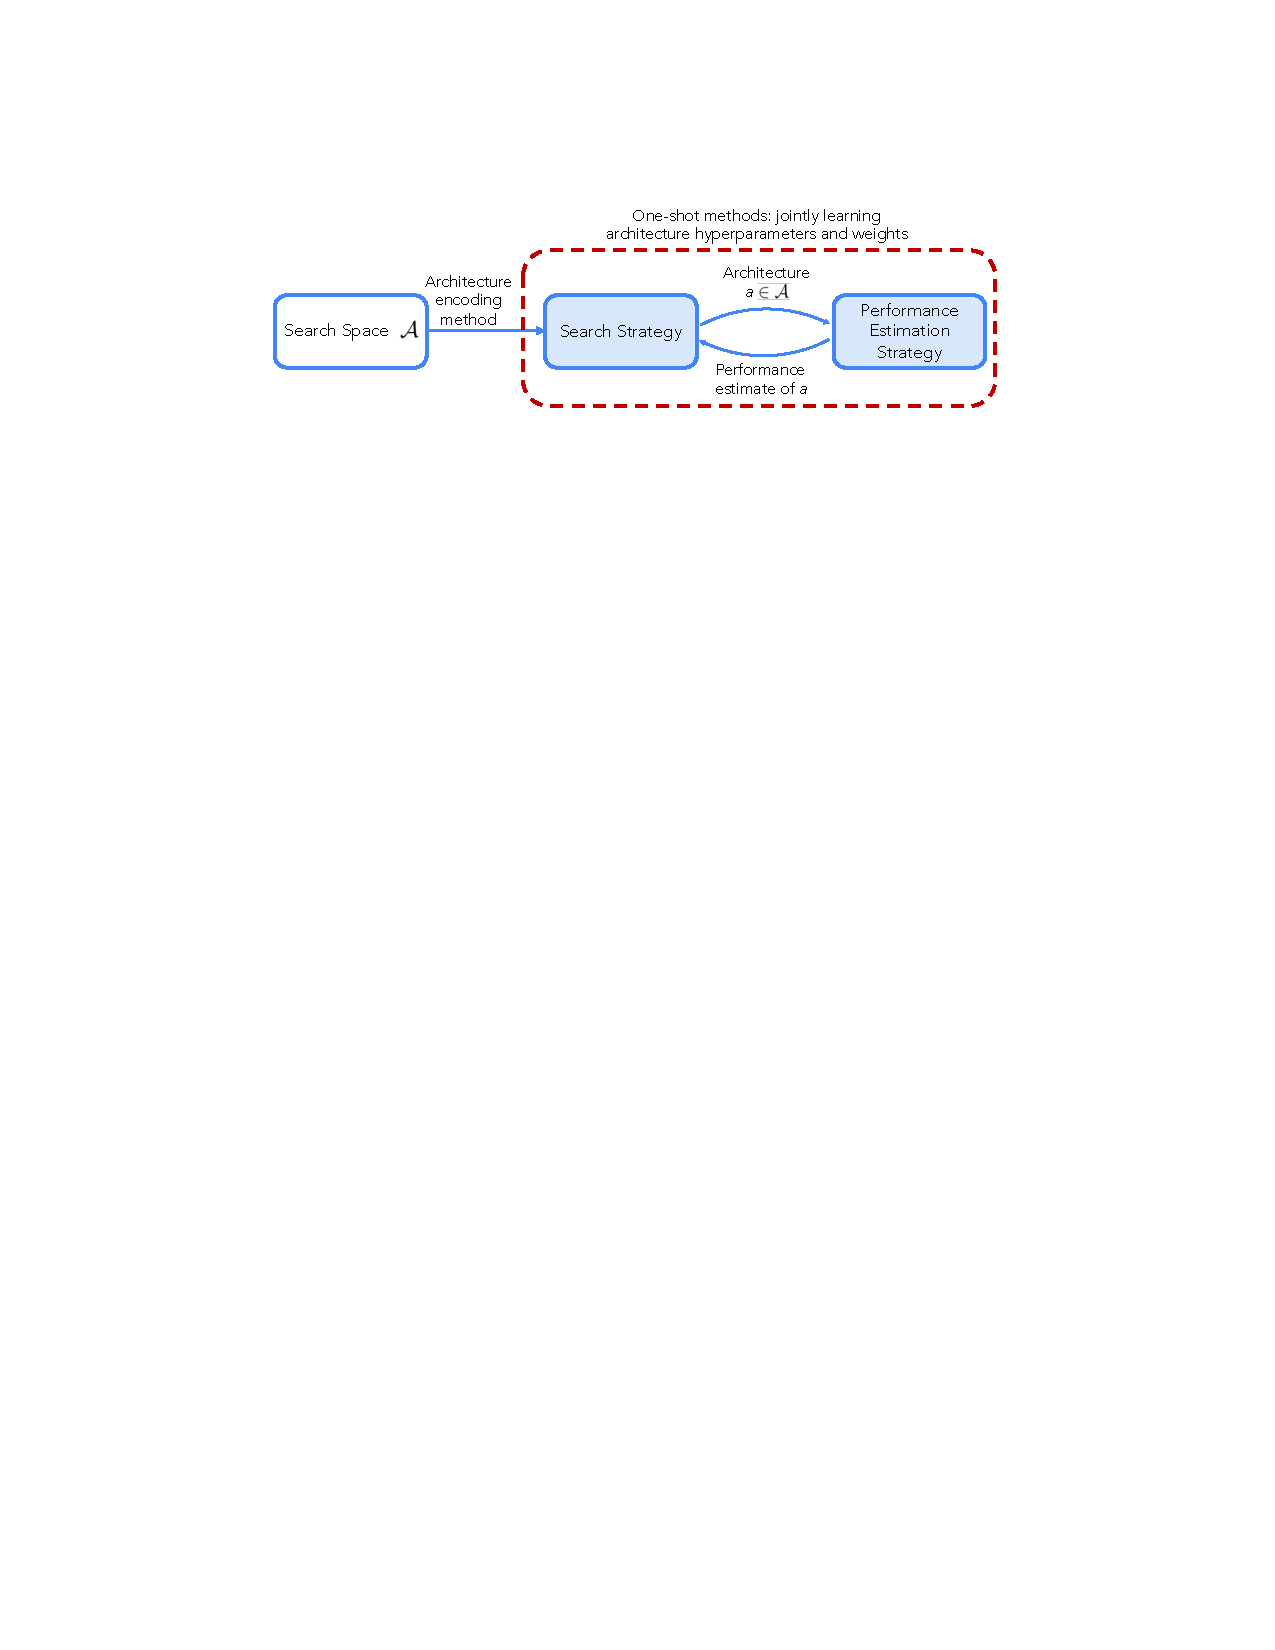
\includegraphics[width=\linewidth]{overview_NAS.pdf}
        \caption{Overview of NAS.

            A search strategy iteratively selects architectures (typically by using an architecture encoding method) from a predened search space $ \mathcal{A} $ .

            The architectures are passed to a performance estimation strategy, which returns the performance estimate to the search strategy.

            For one-shot methods, the search strategy and performance estimation strategy are inherently coupled.}
        % citer le papier 1000
    \end{figure}
\end{frame}

%------------------------------------------------
\subsection{Search space}
\begin{frame}{Search space}
    \begin{columns}[c] % The "c" option specifies centered vertical alignment while the "t" option is used for top vertical alignment
        \column{.6\textwidth}
        \begin{block}{Definition}
            The set of all architectures that the NAS algorithm is allowed to select.
        \end{block}
        \begin{itemize}
            \item Size: from a few thousand to over $ 10^{20} $.
            \item Reduction: adding domain knowledge.
            \item [$\rightarrow$] Introduce humain bias $\rightarrow \xmark $ reduce the chance of finding truly nover architecture.
        \end{itemize}
        % Plein de type de search space, voir papier, nous on veut surtout des DAG pour présenter diffusionNAG
        \column{.4\textwidth}
        \begin{figure}[H]
            \centering
            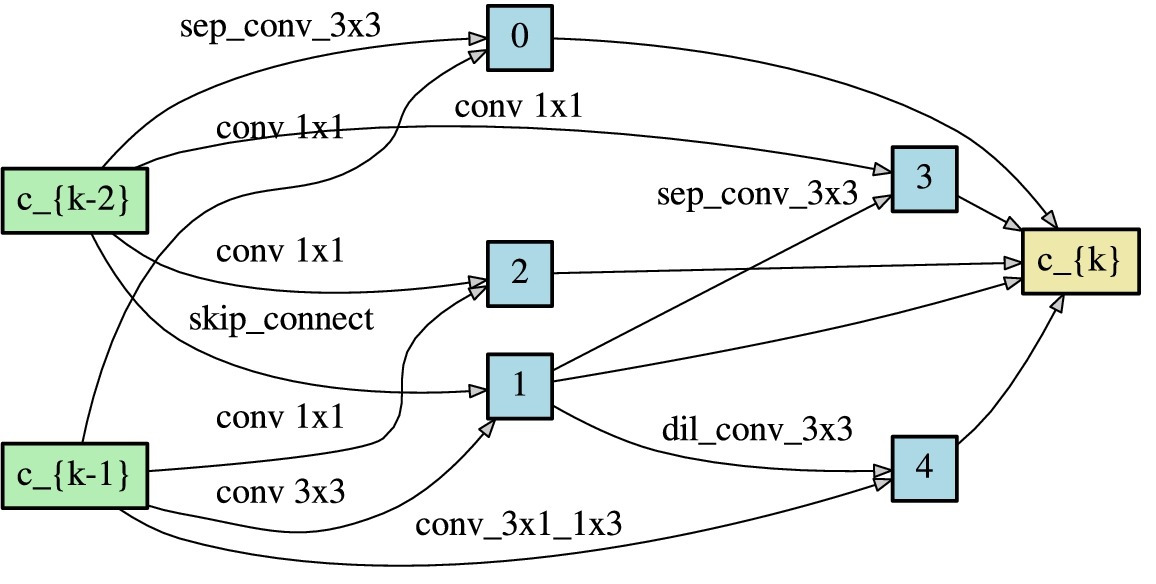
\includegraphics[width=\textwidth]{architecture.jpg} % Mettre la figure 3 page 8 à la place
            \caption{Architecture directed acyclic graph (DAG) with operation on nodes}
        \end{figure}
    \end{columns}
\end{frame}

\subsection{Search strategy}
\begin{frame}{Search strategy}
    \begin{block}{Definition}
        The optimization technique used to find a high-performing architecture in the search space.
    \end{block}
    \begin{itemize}
        \item Black-box optimization techniques : RL, Bayesian optimization, evolutionary search.
        \item One-shot techniques: supernet-hypernet based methods.
    \end{itemize}
    % Naturellement, certaine technique ne rentre dans aucunes des cases 
\end{frame}

\subsection{Performance estimation strategy}
\begin{frame}{Performance estimation strategy}
    \begin{block}{Definition}
        Any method used to quickly predict the performance of neural architectures in order to avoid fully training the architecture.
    \end{block}
    \begin{itemize}
        \item Full training \& evaluation.
        \item Performance estimation strategy.
    \end{itemize}
    \begin{figure}[htbp]
        \centering
        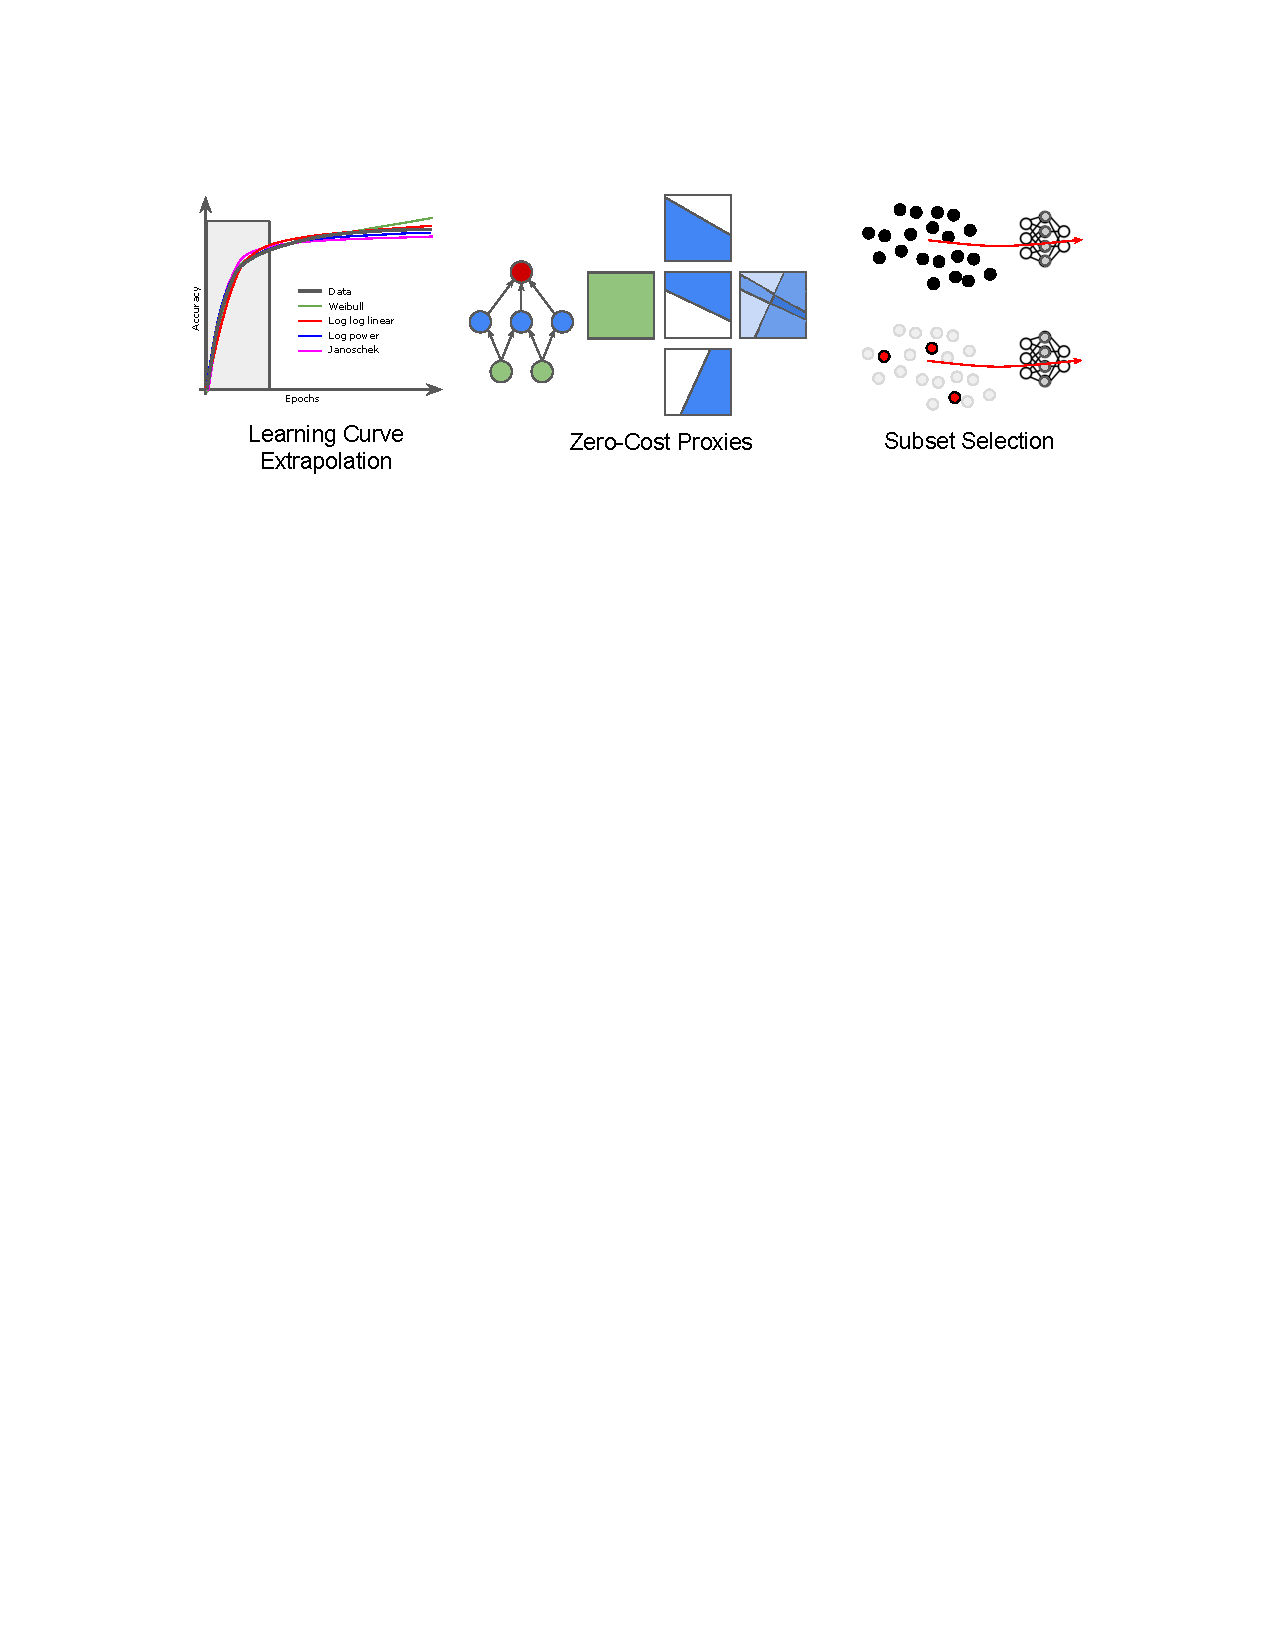
\includegraphics[width=.7\linewidth]{perf_estim_strat.pdf}
        % citer le papier 1000
    \end{figure}
    % parler du meta learning (dernier paragraphe page 26), j'pense c'est proche de difusionNAG 
\end{frame}

%------------------------------------------------
\subsection{Evaluation}
\begin{frame}{Benchmarks}
    %For example, it became standard to train the final architecture for 600 epochs, even though the test accuracy only increases 
    % by a fraction of a percent past 200 epochs. Recently, queryable NAS benchmarks have
    % helped the field reduce computation when developing NAS techniques and to achieve fair,
    % statistically significant comparisons between methods.
    \begin{block}{Definition}
        A NAS benchmark is defined as a dataset with a fixed train-test split, a search space, and a fixed evaluation pipeline for training the architectures.
    \end{block}
    \begin{itemize}
        \item Tabular benchmarks: precomputed evaluations for all possible architecture in the search space.
        \item [$\rightarrow$] Allow to \textbf{simulate} hundreds of trials !\begin{itemize}
                  \item No more training.
                  \item Statistically significant comparisons (simulation with multiple seeds).
              \end{itemize}
        \item Specialization: precomputed evaluation for NLP tasks, protein folding, astronomy imaging, for vision dataset (CIFAR-10(0), ImageNet, ...)
        \item Most popular NAS benchmarks \begin{itemize}
                  \item NAS-Bench-101/202
                  \item Surr-NAS-Bench-DARTS
                  \item TransNAS-Bench-101
                  \item NAS-Bench-Suite
              \end{itemize}
    \end{itemize}
\end{frame}
%------------------------------------------------
\begin{frame}
    \frametitle{Evalutation}
    \begin{figure}[htbp]
        \centering
        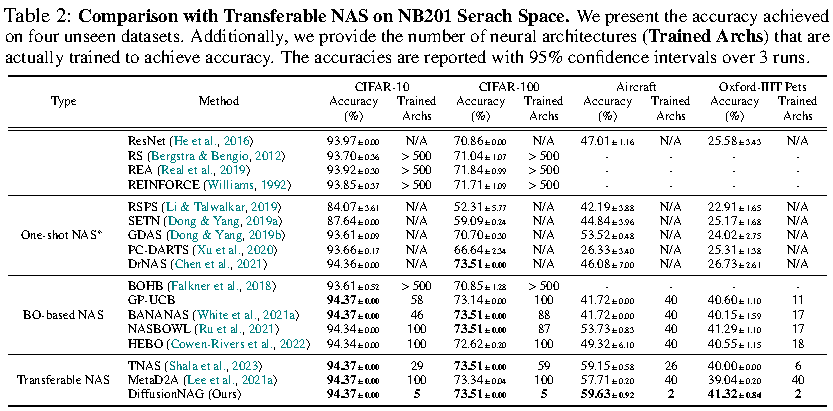
\includegraphics[height=.7\textheight]{table_diffusionNAG.pdf}
        \caption{Result table example}
    \end{figure}
\end{frame}
%------------------------------------------------
\begin{frame}
    \frametitle{Evalutation}
    \begin{figure}[htbp]
        \centering
        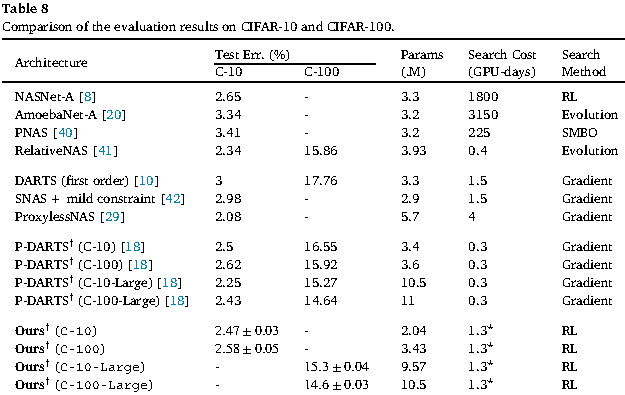
\includegraphics[height=.7\textheight]{table_random.pdf}
        \caption{Result table example}
    \end{figure}
\end{frame}

%------------------------------------------------
\section{Contribution}
%------------------------------------------------

\begin{frame}
    \frametitle{Contribution}
    \framesubtitle{diffusionNAG}
    \begin{itemize}
        \item Problem: Classical NAS need to train thousand of architecture.
        \item [$\rightarrow$] Switch from searching architecture to directly generate architecture using a graph diffusion model.
        \item [$\rightarrow$] diffusionNAG
    \end{itemize}
\end{frame}

\begin{frame}
    \frametitle{Contribution}
    \framesubtitle{diffusionNAG}
    \begin{figure}[htbp]
        \centering
        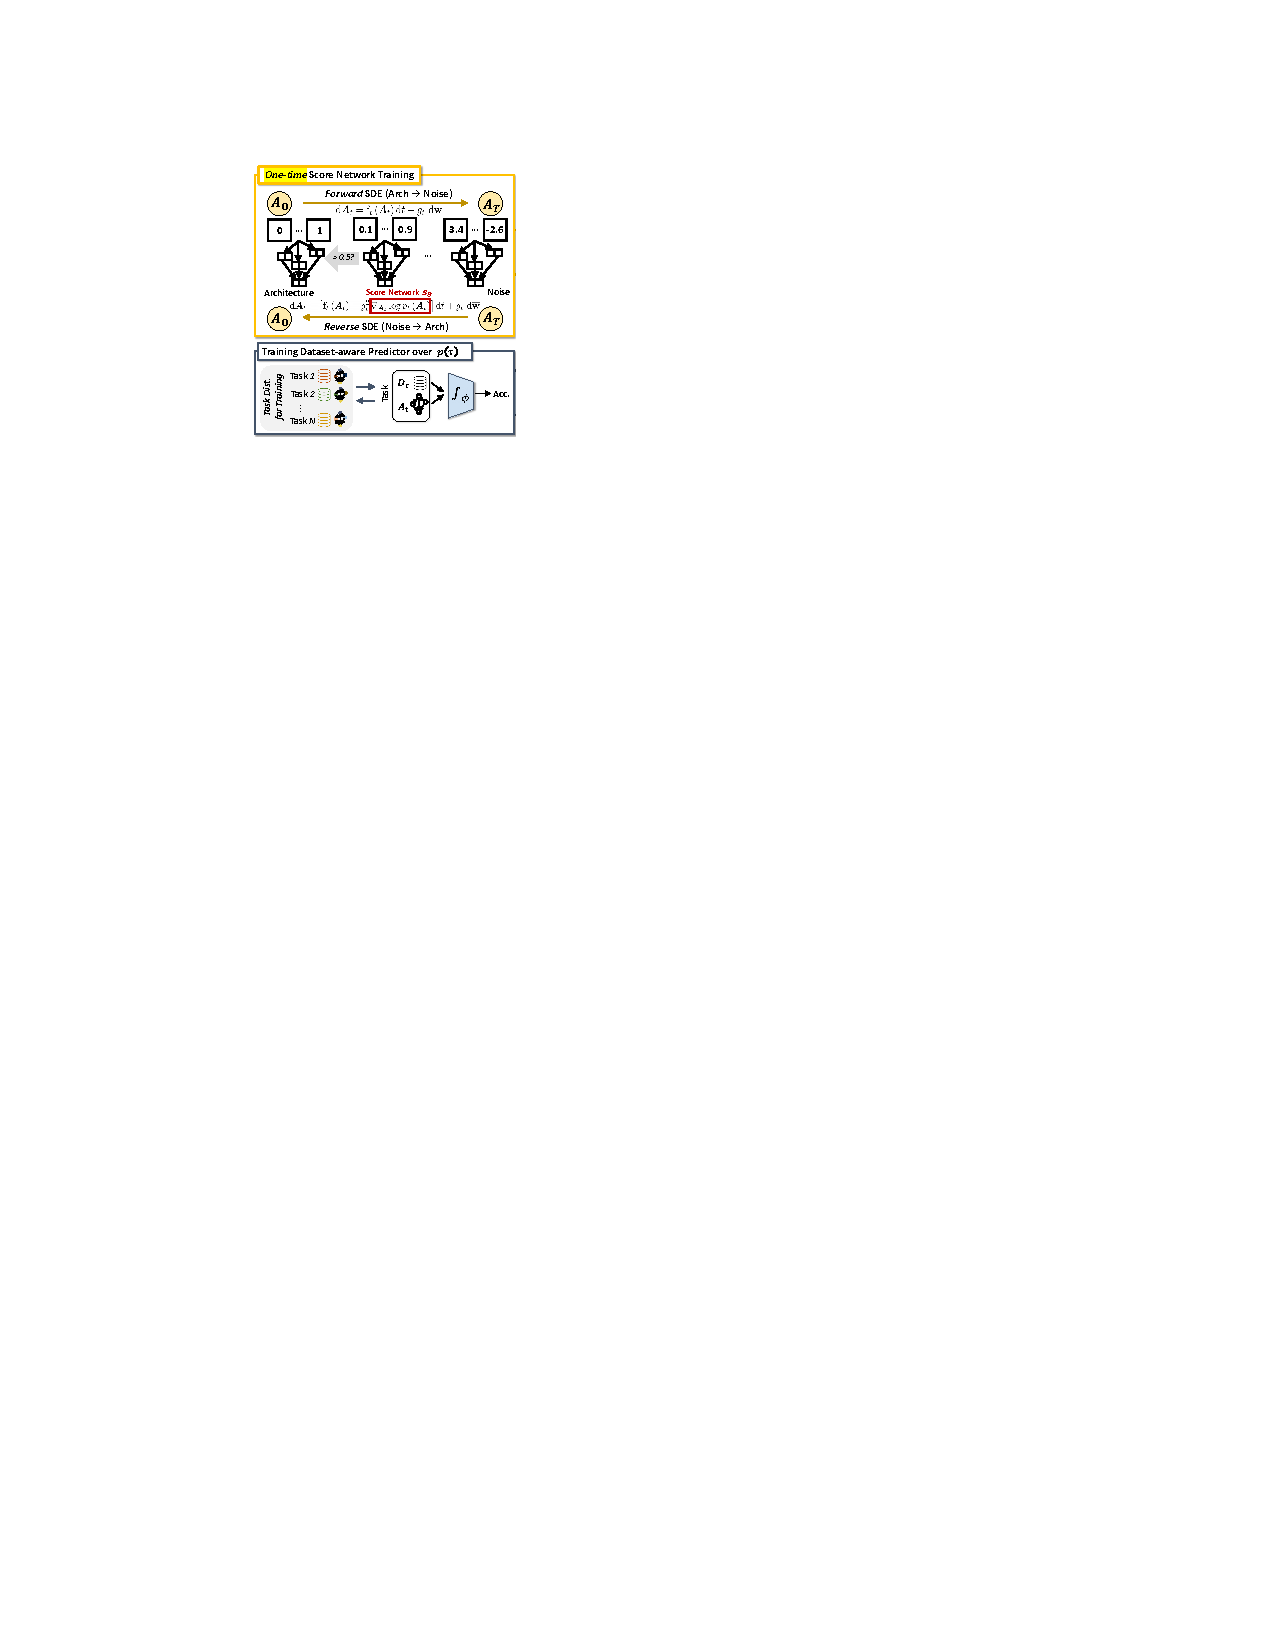
\includegraphics[height=.80\textheight]{diffusionNAG_part1.pdf}
    \end{figure}
\end{frame}

\begin{frame}
    \frametitle{Contribution}
    \framesubtitle{diffusionNAG}
    \begin{figure}[htbp]
        \centering
        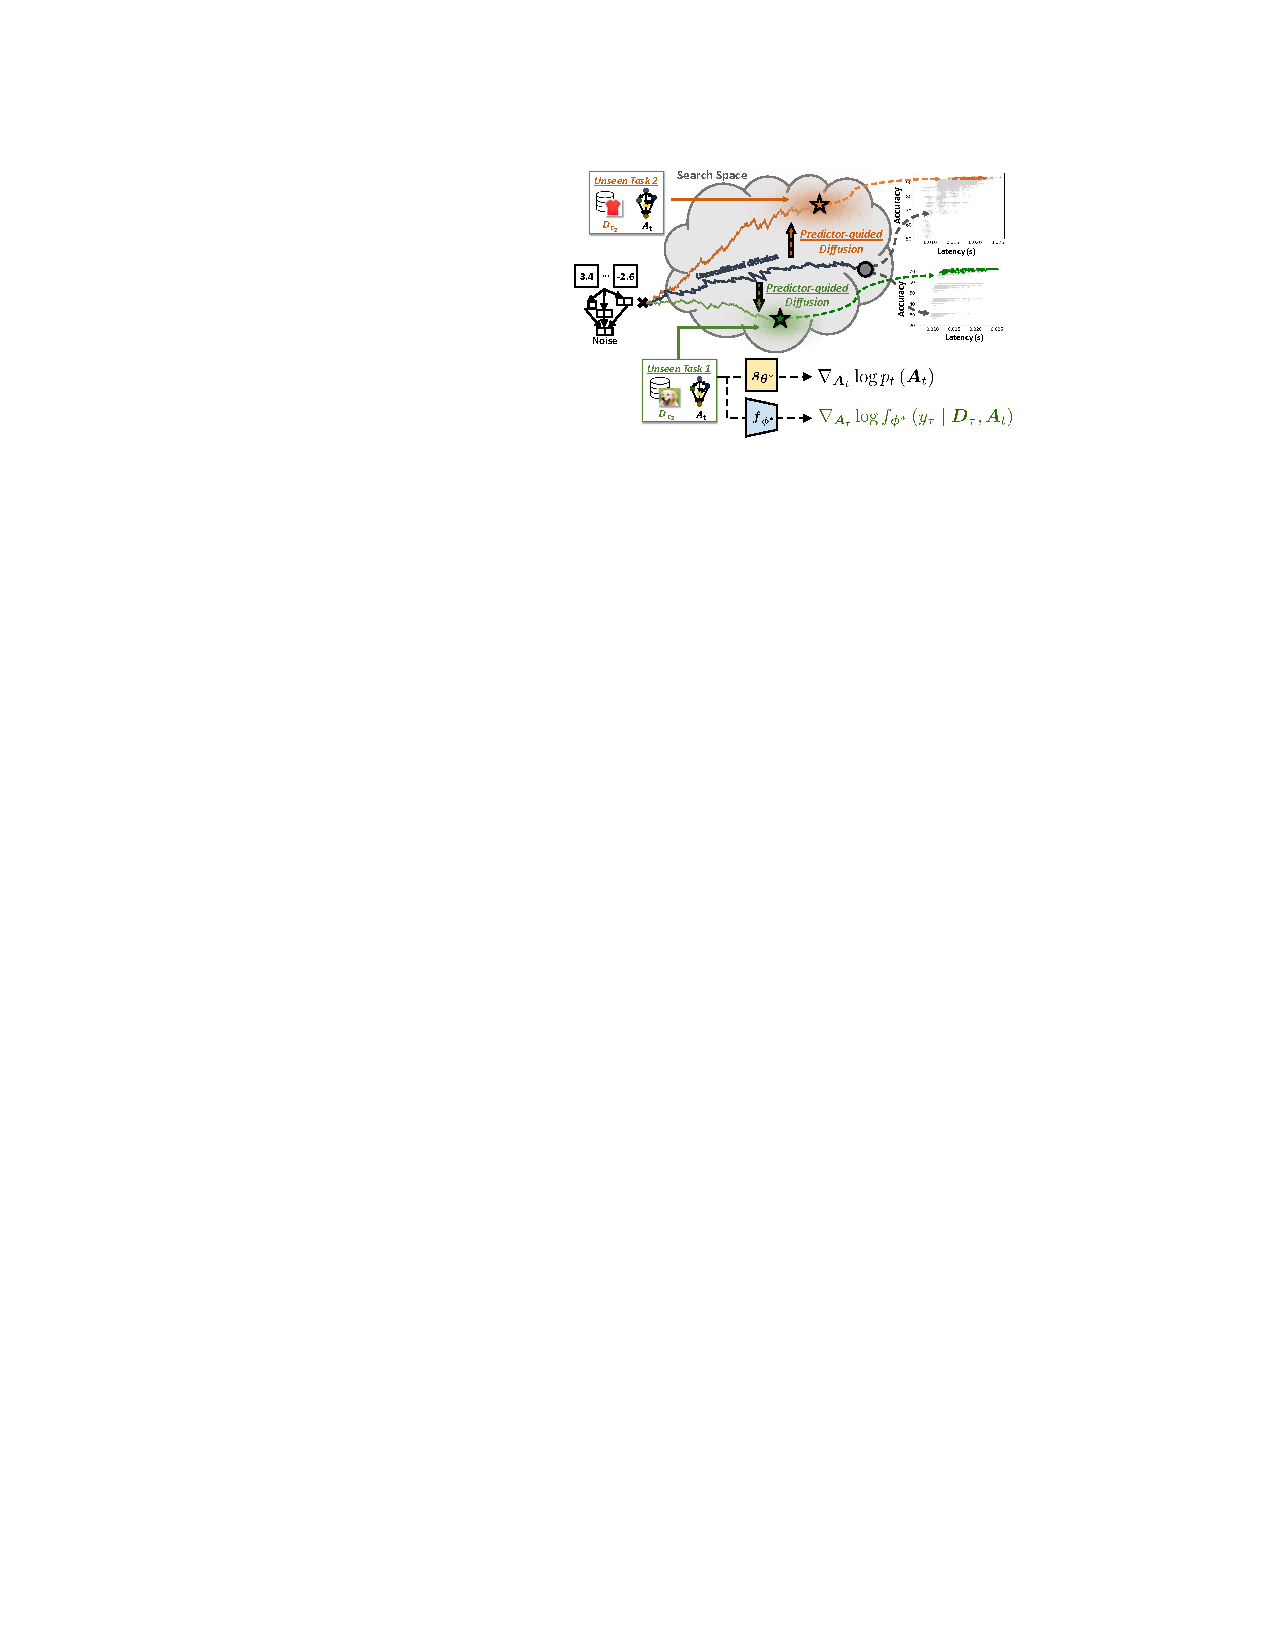
\includegraphics[height=.80\textheight]{diffusionNAG_part2.pdf}
    \end{figure}
\end{frame}
\begin{frame}
    \frametitle{Contribution}
    \framesubtitle{diffusionNAG}
    Limits
    \begin{itemize}
        \item Need to retrain $ f_\Phi $ for every metrics
            \begin{itemize}
                \item Accuracy
                \item Inference time
                \item Memory usage
                \item Adversarial attack resistance
                \item ...
            \end{itemize}
        \item Only one metric is optimized: no compromise possible
        \item Linear combination of metrics: not ideal to find a good compromise
    \end{itemize}
\end{frame}

\begin{frame}{Our contrib title}
    \begin{columns}[c]
        \column{.6\textwidth} % Left column and width
        \begin{itemize}
            \item Train a multi-objective predictor using the same task aware dataset, but enhanced with metrics of interest
            \item Guide the diffusion with the multi-objective predictor:
                \begin{itemize}
                    \item Generate a bigger super-network with disableable blocks
                    \item ie: equal to an encoding of points near the pareto front (best possible compromise between metrics)
                \end{itemize}
            \item Constraints encoding within the same score network
                \begin{itemize}
                    \item Layer compatibility in a block
                    \item Compatibility between blocks inputs and outputs
                \end{itemize}
        \end{itemize}

        \column{.4\textwidth} % Right column and width
        \begin{figure}[htbp]
            \centering
            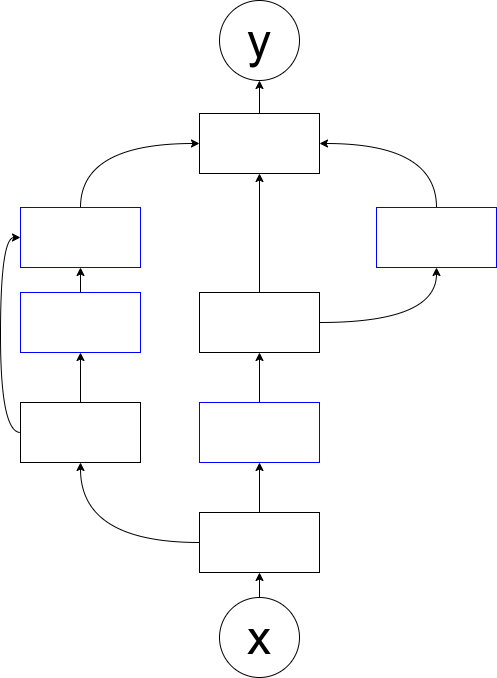
\includegraphics[width=.7\textwidth]{diagram.drawio.png}
            \caption{Example of disableable architecture}
        \end{figure}
    \end{columns}
\end{frame}

\begin{frame}
    \begin{itemize}
        \item Train the obtained super-network after diffusion inference
        \item Disable the blocks depending on the metrics of interest
    \end{itemize}
    % TODO: add archi with transparent / blurred blocks and pareto frontiers
    \begin{columns}[c]
        \column{.45\textwidth} % Left column and width
        \begin{figure}[htbp]
            \centering
            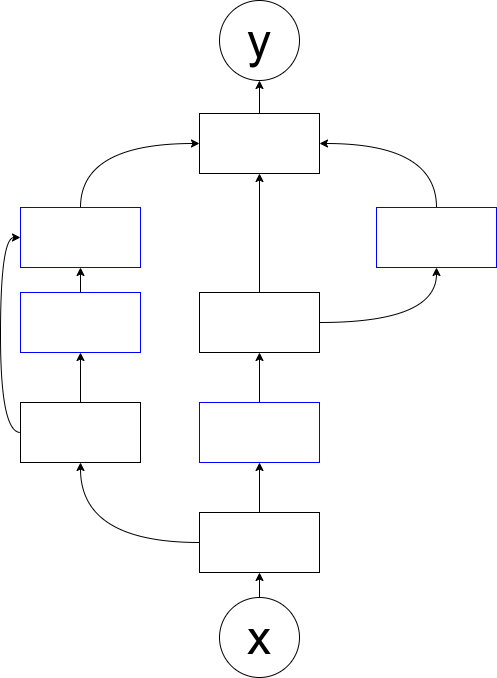
\includegraphics[width=.8\textwidth]{diagram.drawio.png}
        \end{figure}
        \column{.45\textwidth} % Right column and width
        \begin{figure}[htbp]
            \centering
            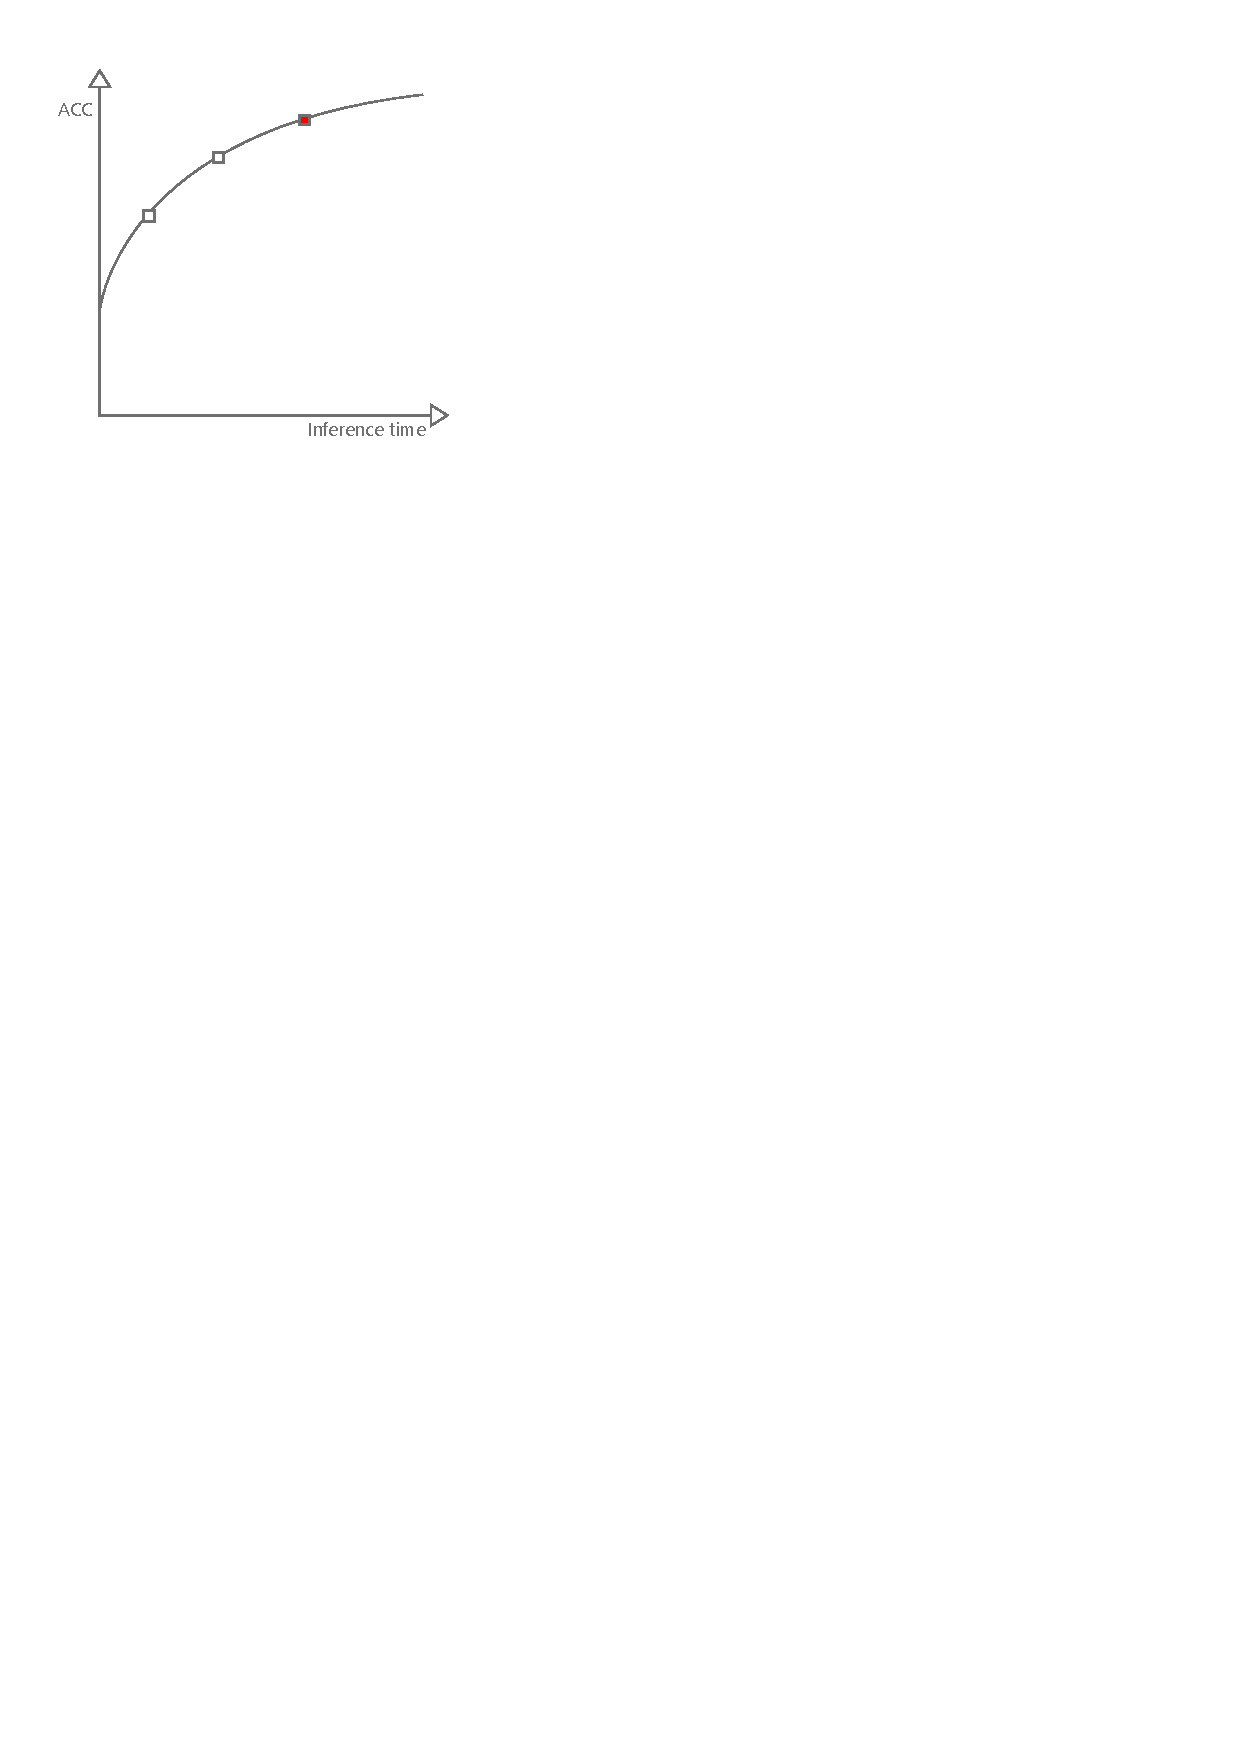
\includegraphics[width=.8\textwidth]{pareto_front.pdf}
        \end{figure}
    \end{columns}
\end{frame}
\begin{frame}
    \begin{itemize}
        \item Train the obtained super-network after diffusion inference
        \item Disable the blocks depending on the metrics of interest
    \end{itemize}
    % TODO: add archi with transparent / blurred blocks and pareto frontiers
    \begin{columns}[c]
        \column{.45\textwidth} % Left column and width
        \begin{figure}[htbp]
            \centering
            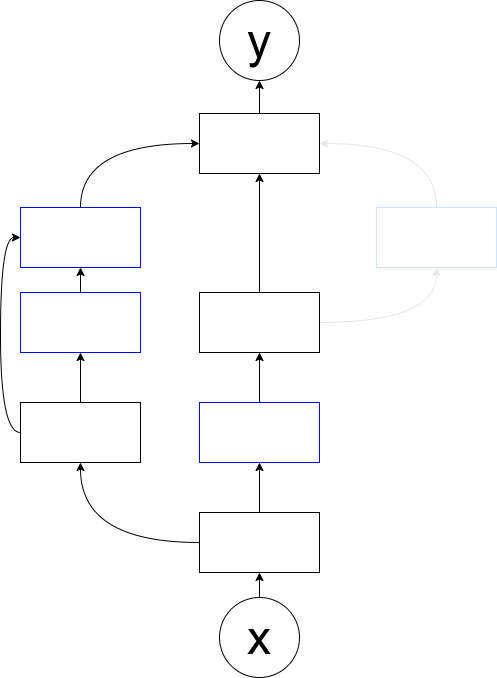
\includegraphics[width=.8\textwidth]{diagram_disabled1.drawio.png}
        \end{figure}
        \column{.45\textwidth} % Right column and width
        \begin{figure}[htbp]
            \centering
            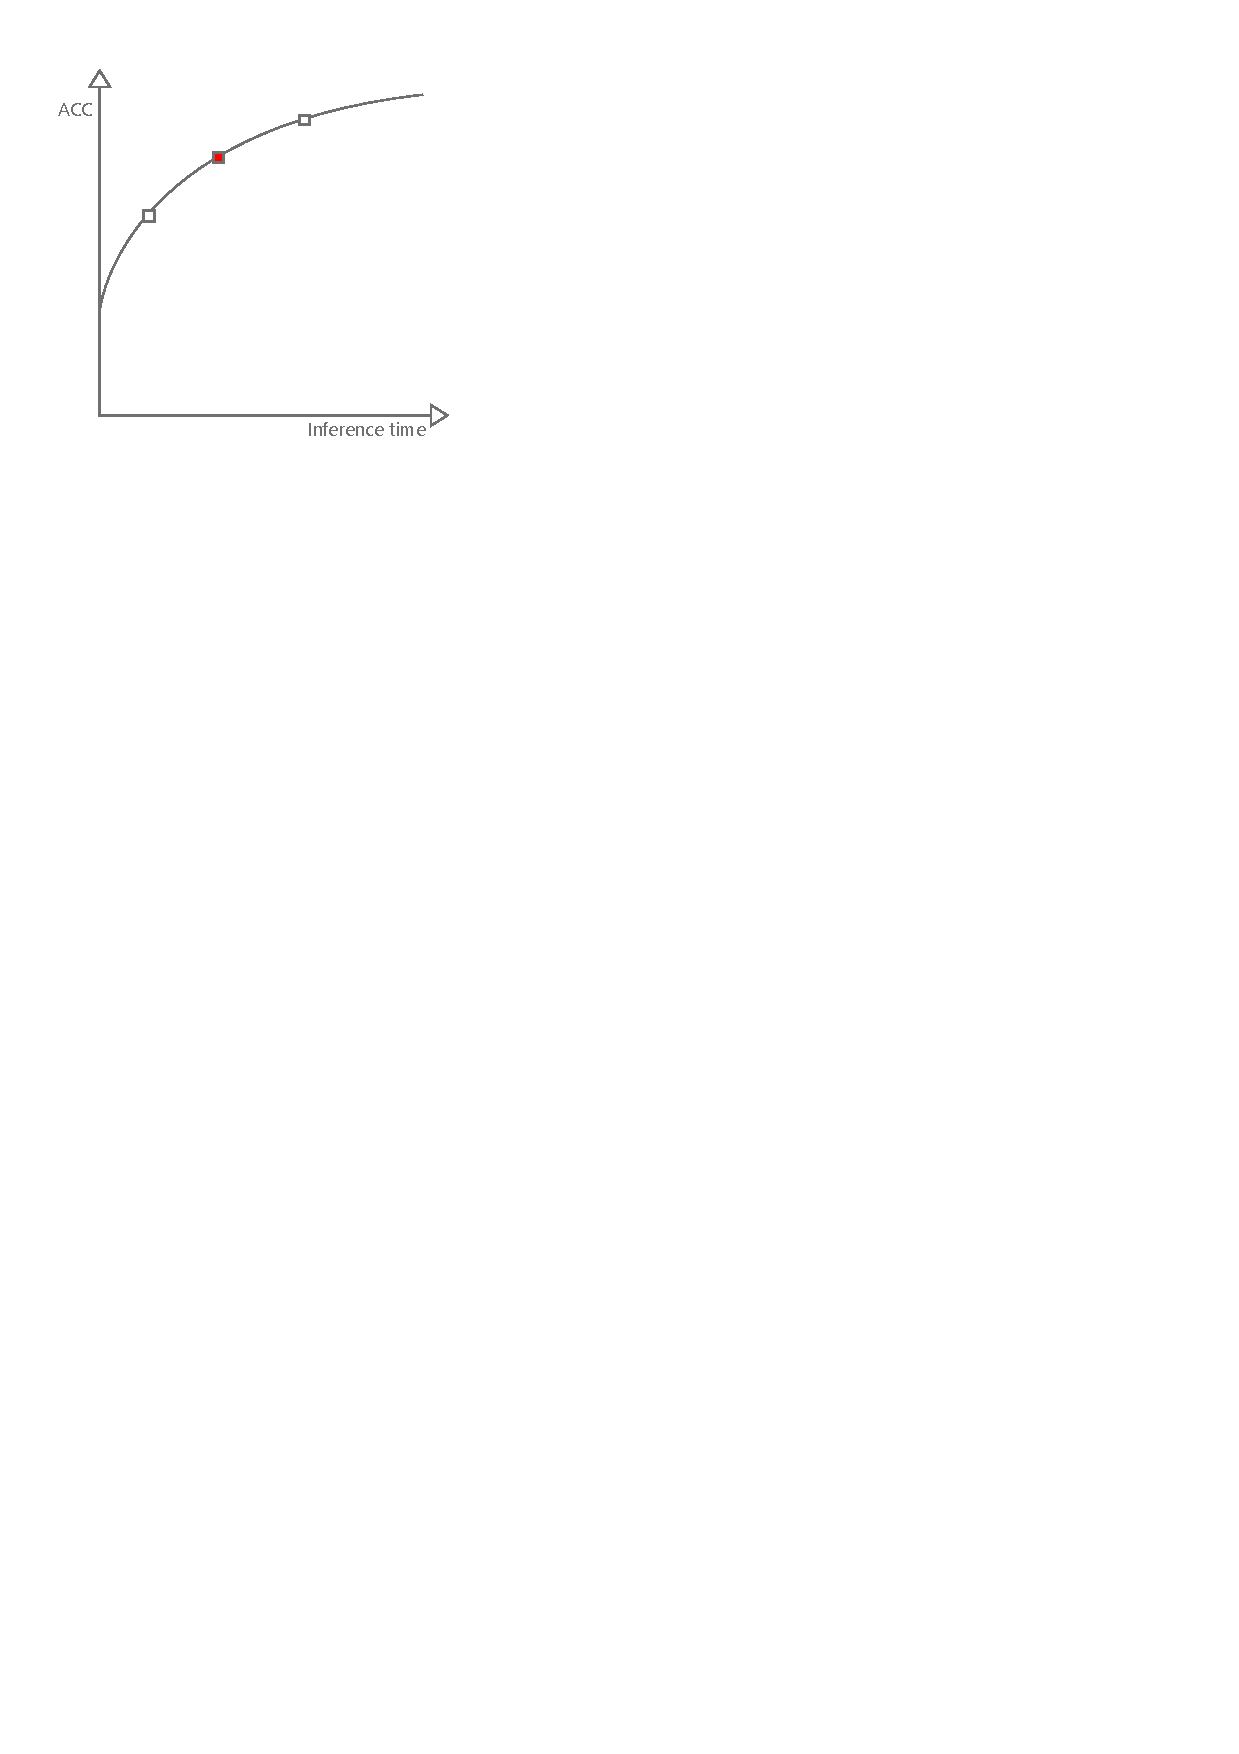
\includegraphics[width=.8\textwidth]{pareto_front_disabled1.pdf}
        \end{figure}
    \end{columns}
\end{frame}
\begin{frame}
    \begin{itemize}
        \item Train the obtained super-network after diffusion inference
        \item Disable the blocks depending on the metrics of interest
    \end{itemize}
    % TODO: add archi with transparent / blurred blocks and pareto frontiers
    \begin{columns}[c]
        \column{.45\textwidth} % Left column and width
        \begin{figure}[htbp]
            \centering
            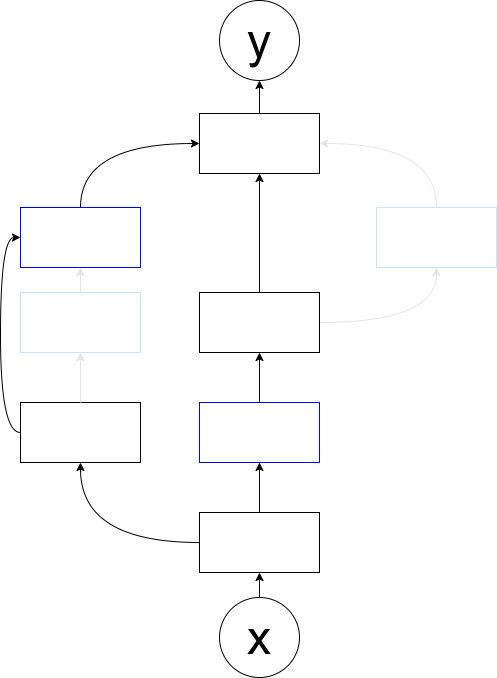
\includegraphics[width=.8\textwidth]{diagram_disabled2.drawio.png}
        \end{figure}
        \column{.45\textwidth} % Right column and width
        \begin{figure}[htbp]
            \centering
            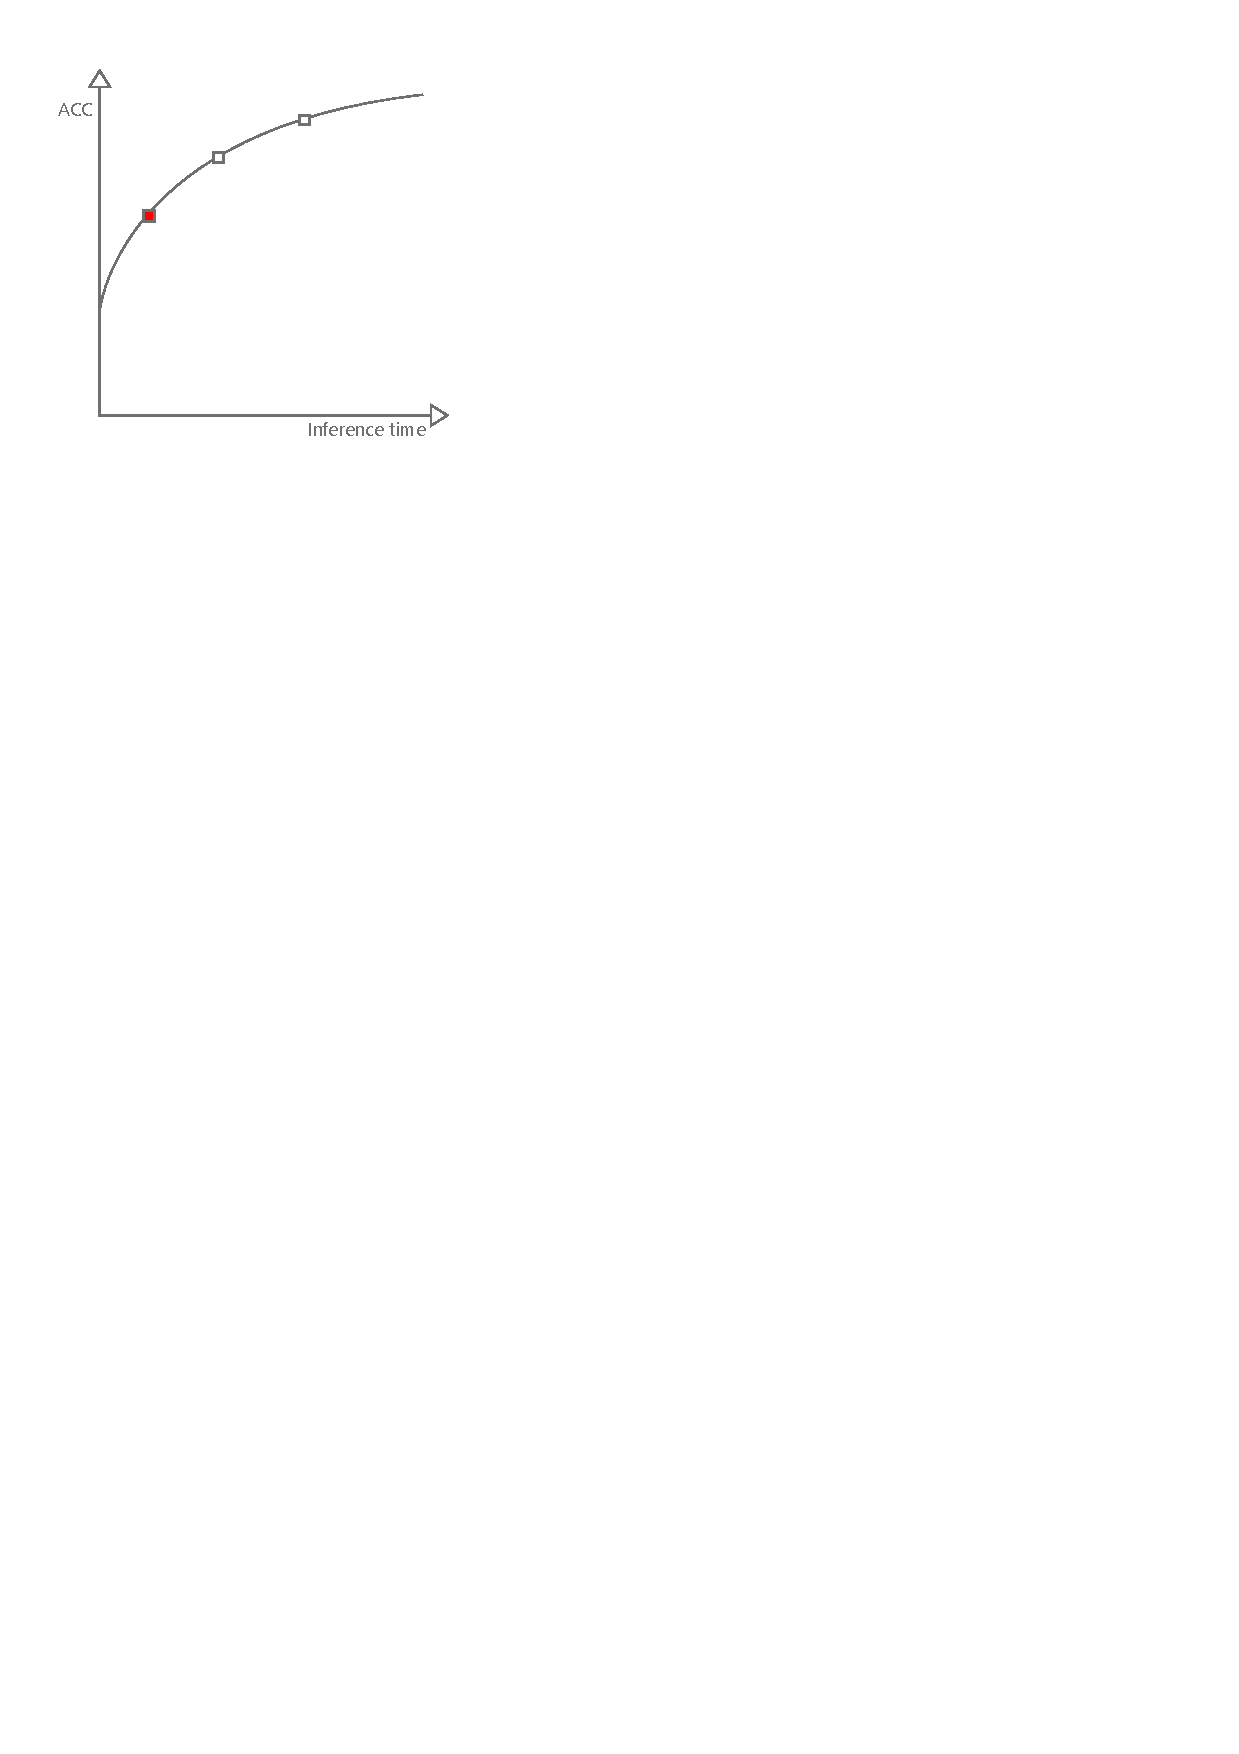
\includegraphics[width=.8\textwidth]{pareto_front_disabled2.pdf}
        \end{figure}
    \end{columns}
\end{frame}

% TODO : add image of our diffusion with pareto frontier

\begin{frame}
    \frametitle{Advantages and limits of this approach}
    \begin{itemize}
        \item Flexibility for the user : fix the metrics threshold only after performing the NAS
        \item Dynamic architecture depending on external parameters
            % energy consumption for a robot in a difficult situation is no longer pertinent
    \item But :
            \begin{itemize}
                \item Predictor needs to be retrained if a new metric is added
                \item Diffusion inference more costly
                \item No guarantees if the pareto optimality is well covered by the disableable blocks
            \end{itemize}
    \end{itemize}
\end{frame}

\begin{frame}{Multi-achitecture search}

    \frametitle{Evaluation and results}
    % \begin{columns}[c] 
    % \column{.45\textwidth} % Left column and width
    \textbf{Two evaluations}
    \begin{itemize}
        \item Achitecture search
        \item generated architecture performances
    \end{itemize}

    \begin{itemize}
        \item generation cheaper than previous full space search
        \item multi-objective benchmarks for the obtained architectures
    \end{itemize}

    % \column{.5\textwidth} % Right column and width

    \begin{tabular}{ |p{3cm}||p{3cm}|p{3cm}|p{3cm}|  }
        \hline
        \multicolumn{4}{|c|}{Results for a classifier model on CIFAr-10}                                      \\
        \hline
        Model                                                  & Ours & DiffusionNAG & (egrg) best RL methods \\
        \hline
        architecture search time (min)                         & 23.6 & 544          & > 2000                 \\
        Inference costs of the generated architecture (MFLOPs) & 250  & 434          & 670                    \\
        \hline
    \end{tabular}

    % \end{columns}
\end{frame}


%------------------------------------------------

\begin{frame}{References}
    % Beamer does not support BibTeX so references must be inserted manually as below
    \footnotesize{
        \begin{thebibliography}{99}
            \bibitem[Smith, 2012]{p1} John Smith (2012)
            \newblock Title of the publication
            \newblock \emph{Journal Name} 12(3), 45 -- 678.
        \end{thebibliography}
    }
\end{frame}

%------------------------------------------------

\begin{frame}
    \Huge{\centerline{\textbf{Thank you}}}
\end{frame}

%----------------------------------------------------------------------------------------

\end{document}

% \begin{frame}[fragile] % Need to use the fragile option when verbatim is used in the slide
%     \frametitle{frame documnetation}
%     An example of the \verb|\cite| command to cite within the presentation:\\~

%     This statement requires citation \cite{p1}.

%     In this slide, some important text will be \alert{highlighted} because it's important. Please, don't abuse it.

%     \begin{block}{Block}
%         Sample text
%     \end{block}

%     \begin{alertblock}{Alertblock}
%         Sample text in red box
%     \end{alertblock}

%     \begin{examples}
%         Sample text in green box. The title of the block is ``Examples".
%     \end{examples}
% \end{frame}
